\documentclass[a4paper, 12pt]{report}
\usepackage[T1]{fontenc} 
% \usepackage[icelandic]{babel}
\usepackage{latexsym,amssymb,amsmath,amsthm}
\usepackage{graphicx}
\usepackage[colorlinks=true,linkcolor=black,anchorcolor=black,citecolor=black,filecolor=black,menucolor=black,runcolor=black,urlcolor=black]{hyperref}
\usepackage{enumerate}
\usepackage{pgfplots}
\usepackage{nicefrac}
\usepackage{derivative}
\usepackage{setspace}
\usepackage{mathrsfs}
%\usepackage{newtxtext, newtxmath}
\usepackage{tabularx}
\usepackage{authblk}
\usepackage{caption}
\usepackage[most]{tcolorbox}

\usepackage{algorithm}
\usepackage{algpseudocodex}
\renewcommand\algorithmicprocedure{\textbf{procedure}}
\newcommand{\algorithmicendprocedure}{\algorithmicend\ \algorithmicprocedure}
\makeatletter
\newcommand\PROCEDURE[3][default]{%
  \ALC@it
  \algorithmicprocedure\ \textsc{#2}(#3)%
  \ALC@com{#1}%
  \begin{ALC@prc}%
}
\newcommand\ENDPROCEDURE{%
  \end{ALC@prc}%
  \ifthenelse{\boolean{ALC@noend}}{}{%
    \ALC@it\algorithmicendprocedure
  }%
}
\newenvironment{ALC@prc}{\begin{ALC@g}}{\end{ALC@g}}
\makeatother


\usepackage[hang,flushmargin]{footmisc}
\captionsetup[figure]{labelfont=bf}


\pgfplotsset{compat=1.17}
\setlength{\jot}{1em}

\title{\textsc{Simulating the Evolution of\\ Neural Pathways and Structures} \\ \vspace*{10mm} \Large Development Journal}
\author[1]{Kári Hlynsson}
\author[2]{Young Jun Lee}
\affil[1]{University of Iceland, Department of Mathematics}
\affil[2]{University of Oxford, Department of Biology}
\date{}

\newtheorem{theorem}{Theorem}[chapter]
\newtheorem{corollary}{Corollary}[chapter]
\newtheorem{proposition}{Proposition}[chapter]

\theoremstyle{definition}
\newtheorem{definition}{Definition}[chapter]
\newtheorem*{remark}{Remark}

\let\oldproofname=\proofname
\renewcommand{\proofname}{\rm\bf{\oldproofname}}


\begin{document}

\maketitle

\onehalfspacing
\newpage

\tableofcontents

\newpage
\chapter*{Index of notation}
\renewcommand{\arraystretch}{1.7}
\begin{table}[ht!]
    \centering
    \begin{tabularx}{\textwidth}{l X}
      \textsc{Abbreviation} & \textsc{Definition} \\
      $\mathscr E = [0;w] \times [0;h]$ & Environment with \emph{width} $w$ and \emph{height} $h$. The environment
                                           can also be expressed as the set of locations $\ell$ such that $\mathscr E = \{\ell := (x, y) \mid x \in [0;w] \land y \in [0;h]\}$ \\
      $n$                                & Size of the population. \\
      $E = (e_x, e_y)$                  & An entity with $x$ and $y$ coordinates in the environment such that $\ell_{E} \in \mathscr E$ ($\ell_E$ is the location which corresponds to the entity's location) \\
      $\mathbf C = \{C_1, \ldots, C_k\}$ & The partition of $\mathscr E$ into $k$ chunks $C_1, \ldots, C_k$ such that $\bigcap_{i = 1}^k C_i = \emptyset$ and $\bigcup_{i = 1}^k C_i = \mathscr E$, i.e. the
                                            \emph{set of chunks} $\mathbf C$ forms a complete partition of $\mathscr E$. \\
      $\mathbf O = \{O_1, \ldots, O_n\}$ & The population, the set of all organisms present within the environment. \\
      $\mathcal P: \mathbf O \to \mathscr E$   & Positional mapping. Returns point representation of an entity's location within $\mathscr E$. Note that $\mathcal P$ is a random variable, which we will
      discuss in more detail in the runtime optimization section. \\
    \end{tabularx}
\end{table}

\newpage
\chapter*{Common Acronyms}
\begin{table}[ht!]
    \centering
    \begin{tabularx}{\textwidth}{l X}
      \textsc{Acronym} & \textsc{Definition} \\
      CBS & Chunk-Based System \\
      UGP & Undirected-Graph Partitioning \\
      BFS & Breadth-First Search
    \end{tabularx}
\end{table}


\newpage

\chapter{Theoretical basis}
\section{Note}
Hello there Jun

\noindent
This is an \textsc{\huge EXTREMELY} primitive draft.

\noindent
None of this final and subject to changes as we cooperate on this project.

\noindent
I also want to apologize for the common abbreviatons section, its a load of cowdung
but I feel we will need this to make our lives easier later on.

\par That's alright!! XD The common abbreviations section is really useful, I'll try to follow your notations
throughout the doc.

\section{Relevant biology}
Neural network, to an extent, mimics the interconnected nerve cells in animals, noting that learning can be achieved by modulating certain
'parameters' that dictates how individual neurones respond to a set of stimuli.

\chapter{Model outline}
\section{Model outline}
\subsection{Overview}
The aim of the model is to study the natural evolution of neural pathways in a population of organism
when exposed to survivalistic conditions. A rigid logical and syntactical foundation will make all succeeding
articulation on the model parameters and attributes easier. We therefore dedicate this first section towards
establishing a foundation of terms and definitions which we build on later.
\par The most critical aspects of the model we define here is the \emph{environment} and the \emph{entities} contained
therein. Neglecting any elevation, we define the environment as the bounded subset of the Cartesian plane, which we symbolize
$\mathscr E$ \footnote{Although elevation certainly plays a vital role in the foraging patterns of organisms in natural environments, we refrain
from its implementation as it only adds a level of complexity to the model design while having no immediate benefit for the simulation.}.
\par Contained within the environment are \emph{entities} which we can think of as actors within the simulation. The two types that occur
in this model are \emph{organisms} and \emph{food}. Again, a simple intuitive definition is that the organism is an individual of a species
present within the environment and nutrition is the foodstuffs which it consumes to gain energy and thus survive.
\par Entities can be divided into two types: \emph{organisms} and \emph{food}. What follows is simple: organisms are motile, can sense their surroundings
and consume food to gain energy. On the other hand, food has none of these qualities. We represent an entity as the object $E$, while organisms are denoted
$O$ and food by $F$.
\begin{figure}
    \centering 
    \begin{tcolorbox}[colframe = black, colback = white, sharp corners]
        \begin{tikzpicture}[scale = 1, x=0.6pt,y=0.6pt,yscale=-1,xscale=1]
            %uncomment if require: \path (0,300); %set diagram left start at 0, and has height of 300

            %Shape: Circle [id:dp5046571963675113] 
            \draw  [fill={rgb, 255:red, 232; green, 210; blue, 255 }  ,fill opacity=1 ] (169,165.75) .. controls (169,157.05) and (176.05,150) .. (184.75,150) .. controls (193.45,150) and (200.5,157.05) .. (200.5,165.75) .. controls (200.5,174.45) and (193.45,181.5) .. (184.75,181.5) .. controls (176.05,181.5) and (169,174.45) .. (169,165.75) -- cycle ;
            %Shape: Pie [id:dp6264332812271176] 
            \draw   (222.96,129.08) .. controls (225.08,130.35) and (227.1,131.82) .. (229.01,133.51) .. controls (246.31,148.81) and (247.57,175.65) .. (231.82,193.45) .. controls (230.18,195.31) and (228.42,196.99) .. (226.56,198.5) -- (200.5,165.75) -- cycle ;
            %Straight Lines [id:da5980112219613951] 
            \draw [color={rgb, 255:red, 0; green, 0; blue, 0 }  ,draw opacity=1 ]   (200.5,165.75) -- (241,165.27) ;
            \draw [shift={(243,165.25)}, rotate = 179.33] [color={rgb, 255:red, 0; green, 0; blue, 0 }  ,draw opacity=1 ][line width=0.75]    (4.37,-1.32) .. controls (2.78,-0.56) and (1.32,-0.12) .. (0,0) .. controls (1.32,0.12) and (2.78,0.56) .. (4.37,1.32)   ;
            %Curve Lines [id:da9973990148186489] 
            \draw  [dash pattern={on 4.5pt off 4.5pt}]  (2,150) .. controls (42,120) and (103,168) .. (169,165.75) ;
            %Shape: Triangle [id:dp44009432397165527] 
            \draw  [fill={rgb, 255:red, 179; green, 249; blue, 182 }  ,fill opacity=1 ] (324.11,89) -- (338,111) -- (311,111) -- cycle ;

            %Shape: Triangle [id:dp35563504351381514] 
            \draw  [fill={rgb, 255:red, 179; green, 249; blue, 182 }  ,fill opacity=1 ] (600.11,244) -- (614,266) -- (587,266) -- cycle ;

            %Shape: Triangle [id:dp6587382072289927] 
            \draw  [fill={rgb, 255:red, 179; green, 249; blue, 182 }  ,fill opacity=1 ] (585.11,47) -- (599,69) -- (572,69) -- cycle ;

            %Shape: Triangle [id:dp8230417371681578] 
            \draw  [fill={rgb, 255:red, 179; green, 249; blue, 182 }  ,fill opacity=1 ] (416.11,221) -- (430,243) -- (403,243) -- cycle ;

            %Shape: Triangle [id:dp3619204635470774] 
            \draw  [fill={rgb, 255:red, 179; green, 249; blue, 182 }  ,fill opacity=1 ] (121.11,55) -- (135,77) -- (108,77) -- cycle ;

            %Shape: Triangle [id:dp9744597746822374] 
            \draw  [fill={rgb, 255:red, 179; green, 249; blue, 182 }  ,fill opacity=1 ] (110.11,227) -- (124,249) -- (97,249) -- cycle ;

            %Shape: Circle [id:dp2625952541482832] 
            \draw  [fill={rgb, 255:red, 232; green, 210; blue, 255 }  ,fill opacity=1 ] (483.04,47.77) .. controls (489.39,53.72) and (489.71,63.68) .. (483.76,70.03) .. controls (477.81,76.38) and (467.85,76.7) .. (461.5,70.75) .. controls (455.15,64.8) and (454.83,54.83) .. (460.78,48.49) .. controls (466.73,42.14) and (476.7,41.82) .. (483.04,47.77) -- cycle ;
            %Shape: Pie [id:dp25830448813204976] 
            \draw   (472.89,112.22) .. controls (470.52,112.89) and (468.06,113.36) .. (465.52,113.6) .. controls (442.53,115.76) and (422.09,98.32) .. (419.87,74.66) .. controls (419.64,72.19) and (419.61,69.75) .. (419.78,67.36) -- (461.5,70.75) -- cycle ;
            %Straight Lines [id:da5039204955567191] 
            \draw [color={rgb, 255:red, 0; green, 0; blue, 0 }  ,draw opacity=1 ]   (461.5,70.75) -- (434.15,100.62) ;
            \draw [shift={(432.8,102.1)}, rotate = 312.48] [color={rgb, 255:red, 0; green, 0; blue, 0 }  ,draw opacity=1 ][line width=0.75]    (4.37,-1.32) .. controls (2.78,-0.56) and (1.32,-0.12) .. (0,0) .. controls (1.32,0.12) and (2.78,0.56) .. (4.37,1.32)   ;
            %Curve Lines [id:da7361275969659062] 
            \draw  [dash pattern={on 4.5pt off 4.5pt}]  (483,47.67) .. controls (512,16.67) and (562,36.67) .. (565,1.67) ;

            % Text Node
            \draw (5,8.4) node [anchor=north west][inner sep=0.75pt]  [font=\LARGE]  {$\mathscr{E}$};
            % Text Node
            \draw (320,97.4) node [anchor=north west][inner sep=0.75pt]  [font=\scriptsize]  {F};
            % Text Node
            \draw (596,252.4) node [anchor=north west][inner sep=0.75pt]  [font=\scriptsize]  {F};
            % Text Node
            \draw (581,55.4) node [anchor=north west][inner sep=0.75pt]  [font=\scriptsize]  {F};
            % Text Node
            \draw (412,229.4) node [anchor=north west][inner sep=0.75pt]  [font=\scriptsize]  {F};
            % Text Node
            \draw (117,63.4) node [anchor=north west][inner sep=0.75pt]  [font=\scriptsize]  {F};
            % Text Node
            \draw (106,235.4) node [anchor=north west][inner sep=0.75pt]  [font=\scriptsize]  {F};
            % Text Node
            \draw (246,158) node [anchor=north west][inner sep=0.75pt]  [font=\small]  {$\theta$};
            % Text Node
            \draw (177,157.07) node [anchor=north west][inner sep=0.75pt]    {$O$};
        \end{tikzpicture}
    \end{tcolorbox}
    \caption{An illustration of the model} \label{fig:model_illustration}
\end{figure}

\subsection{Sensory mapping of organisms}
One of the key characteristics of organisms is that they are able to sense their proximal surroundings and base their succeeding actions on the information they
have gathered on the environment. In this section we aim to establish a mathematical and syntactical foundation describing the sensory capabilities of organisms
which allows passing environmental data to the organism's neural network.
\par A convenient and well established method of sensory mapping is obtained through the use of \emph{raycasting} or \emph{raylines}, where several line segments
originating from the organism's point location are used as collision sensors which serve as sensors for distance. By calculating the distance of the intersection between
some rayline emitted by an organism and an entity in the field, a metric describing the \emph{sensory depth} from the organism to another entity is established. 

\begin{definition}[Ray set]
    Let $\lambda \in \mathbb R^+$. Suppose that an organism $O$ in an environment $\mathscr E$ with a present entity set $\mathbf E$ has the forward
    facing angle $\theta$ (see figure \ref{fig:model_illustration}). We define the \emph{ray set} of the organism as the linear space vector $\mathbf R = \{r_1, \ldots, r_{\nu_{\mathbf R}}\}$ from $\left[\theta - \Delta_{\mathbf R}; \theta + \Delta_{\mathbf R}\right]$
    numbering $\nu_{\mathbf R}$ elements ($\nu_{\mathbf R}$ is called the \emph{ray number}). Furthermore, we define the quantity $\mathcal S_{\mathbf R} = 2 \Delta_{\mathbf R}$ as the \emph{span} of the ray set.
\end{definition}

\begin{definition}[Ray map]
   The vector function $R_{\lambda}$ is the \emph{ray map} from the ray set $\mathbf R$ to the family of vectors bounded within the organism's sensory field.
   Furthermore, it is defined by
   \[
        R_{\lambda}(r) = \left\langle R_\lambda^x, R_\lambda^y \right\rangle = \langle \lambda \cos r, \lambda \sin r \rangle
   \]
    Where $\lambda$ is the \emph{maximum sensory depth}, i.e. the radius of the sensory field.
\end{definition}

\begin{remark}
    Note that
    \[
        |R_\lambda(r)|^2 = \left(R_\lambda^x\right)^2 + \left(R_\lambda^y\right)^2 = \lambda^2
    \]
    The vector function is the parametrization of a circle sector in the range $\left[\theta - \Delta_{\mathbf R}; \theta + \Delta_{\mathbf R}\right]$
    and the ray set $\mathbf R$ returns a finite collection of vectors with their endpoints located on the arc of the sector.
\end{remark}

\begin{definition}[Sensory field]
    The sensory field of an organism $O$ is the set of vectors $\mathbf S = \{\vec{s}_1, \ldots, \vec{s}_{\nu_{\mathbf R}}\}$ which is returned by the ray map $R_\lambda$ acting on the
    ray set $\mathbf R$. The \emph{maximum sensory depth} is the parameter $\lambda$ which describes the length of the vectors, i.e. $\forall \vec{s}_i \in \mathbf S: |\vec{s}_i| = \lambda$.
\end{definition}

Sensory activation occurs when an entity intersects with the line segment formed by a ray. This can be formalized as the predice $\kappa_{r_i}(E)$

\section{Simulation phases}
For your contemplation (Jun, if you're reading this): I've thought of dividing the simulation into a \emph{foraging phase}, where organisms roam around and collect food.
If they don't get any or deplete their energy, they die. Once the foraging phase is over, the \emph{reproductive phase} starts, where remaining energy is a measure of how
likely organisms are to find a partner and reproduce (this is of course a simplication, there are many other ways to go about this I'm sure). This way, we don't have to make
the reproduction itself an extreme pain (organisms having to find each other, etc.) This would mean that the reproductive phase is not carried out in the "plane" where the simulation
occurs but rather "off screen" where its just a bunch of calculations really.
\par On the other hand it might make for some really interesting data if we were to assign individuals genders and they would map their current energy level and the gender of individuals
in their sensory field and allow for them to reproduce "in the field" lol. Let me know what you think!

Hi Kari - sorry that I only got to have a look at the document now! Those two alternative strategies are similar to what I've been thinking about as well. 
\par I suppose if we are doing the 'on-screen reproduction' strategy, we'll somehow have to enable agents to switch from \emph{foraging phase} to \emph{reproductive phase};
perhaps by having two different sets of neural networks? I think it's definitely worth developing but I think in this case we would need to consider a way
in which we can ensure agents all dying without offsprings in generation 1 due to incompetence in finding partners.
\par The 'off-screen reproduction' is certainly easier - perhaps we can make an algorithm that randomly picks two individuals with probability of selection
being scaled according to the amount of food collected over their lifetime? This might be possible if we use an algorithm that's kind of like the following:
\par 1) Sort the individuals by the amount of food they have collected (or the energy 'left over' at the end of the foraging phase if foraging also involves
some kind of energy expenditure); 2) Calculate 'boundary values' that divides, for example, [0,1) into sub-intervals proportional to the amount of food
individuals have collected (e.g. if there are two individuals that each collected 3 and 1 amounts of food, subdivide [0,1) into
[0,0.75) and [0.75,1) ); 3) Generate a random number between [0,1); 4) Determine which sub-interval the number falls into, and select the corresponding individual
\par Using this, we should be able to preferrentially select the most 'fittest' individuals and allow them to mate. Once the sub-intervals have been calculated,
selecting more individuals for additional mating shouldn't be too costly computationally speaking (But let me know what you think!)


\section{Runtime optimization}
One of the run-ins we've had so far is determining how to design the sensory mapping capabilities of organisms within the environment. By sensory mapping, I am referring to the organism's ability to sense its
proximal surroundings, sensing the proximity and types of the various entities they may encounter. This will be fed into their neural network, which outputs some response which instructs the organism how to behave
given its current surroundings.
\par The first attempt I made was in the days where the environment was grid-based instead of a float-based environment. There, sensory mapping was quite easy as all that had to be done was inspect the proximal tiles
and check for the entity type present in the tile. This is not possible in the float-based environment, so we propose another solution.
\par An excellent idea you came up with was the idea of partitioning the environment into separate chunks, which organisms restrict their sensory mapping to unless there sensory fields intersect another adjacent chunk
(more on that later). We will start by discussing this idea, which as you will see, will be of great use.

\subsection{Chunk system}
In this section, we will be doing a mathematical analysis of the chunk system to see how it will benefit the simulation. To start off, we inspect what fundamental laws apply to this system.

\begin{proposition}
    Let $\mathscr E$ be an environment paritioned into $k$ chunks such that $\mathbf C = \{C_1, \ldots, C_k\}$. The probability of an entity being present in a generic chunk $C_i$ equals $1/k$, i.e.
    \[
        \textnormal{Pr}\{E \in C_i\} = \frac 1k
    \]
\end{proposition}

\begin{proof}
    Let $\mathscr E$ be the space $[0; w] \times [0;h]$ with $\text{area}(\mathscr E) = wh$ and the partition $\mathbf C$. Under the assumption that the chunks
    are of uniform size, we assume
    \[
        \text{area}(C_i) = \frac{\text{area}(\mathscr E)}{k} \tag{\textasteriskcentered}
    \]
    for all $C_i \in \mathbf C$ where $i \in [1; k]$. Under conventional probability theory, we can express the probability of an entity being in a generic chunk as
    the area of that particular chunk over the area of the environment, i.e.
    \begin{align*}
        \text{Pr}\{E \in C_i\} &= \frac{|C_i|}{|\mathscr E|} \\
                               &= \frac{\text{area}(C_i)}{\text{area}(\mathscr E)} \\
                               &= \frac{1}{k}
    \end{align*}
    The result of the calculations above are immediate of the definition of the area of the chunks, which is derived in (\textasteriskcentered).
\end{proof}

\begin{definition}[Chunk load]
    The random variable $\mathcal L$, or the \emph{chunk load} of some generic chunk $C_i$,
    denotes the number of entities contained within the chunk. Immediate of proposition 1,
    we have that $\mathcal L \sim \text{Bin}(n, 1/k)$, where $n$ is the total number of entities
    in the environment. \footnote{Note that this assumes the uniform distribution of entities within
    the environment. While it not entirely safe to say that the distribution of entities is always uniform, we do so in order to create some upper bound for simulation time}
\end{definition}

\begin{figure}[ht!]
    \centering
    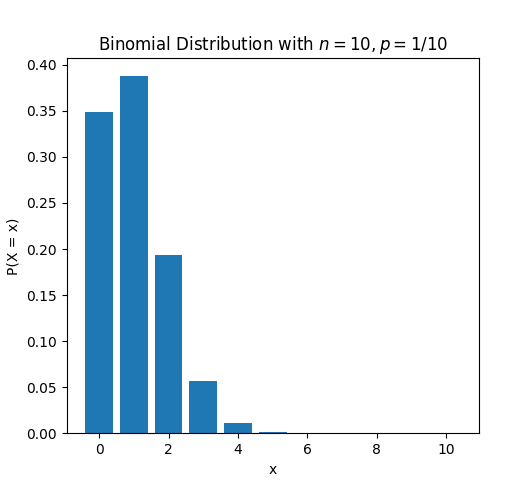
\includegraphics[width=0.9\textwidth]{img/binomialdistribution.png}
    \caption{An example binomial distribution}
\end{figure}

\noindent The random variables $\mathcal L_{C_1}, \ldots, \mathcal L_{C_k}$ are dependent, which by inference leads to $\sum_{i = 1}^k \mathcal L_{C_i} = N$, where $|\mathbf E| = N$. Algorithm \ref*{cbs-costmodel} shows a method with which a amortized cost model can be simulated.
\par The algorithm demands the assignment of $\mathcal L_{C_i}$ for chunks $C_i \in \mathbf C$ by a random process. However, given the nature of probabilistic distributions of dependent variables, 
\begin{figure}[ht!]
    \centering
    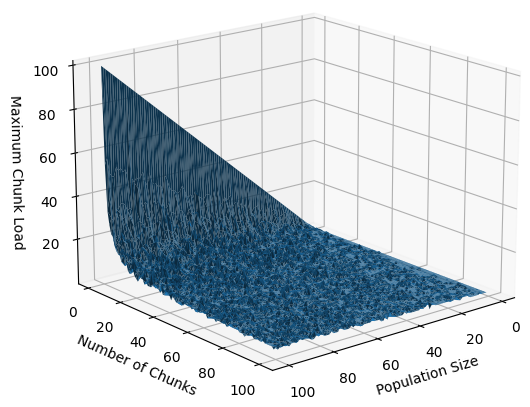
\includegraphics[width=0.9\textwidth]{img/mcl_simulation.png}
    \caption{$\mathcal L_{\max}$ by population size and number of chunks}
\end{figure}

\section{Adjacent chunk loading and critical boundary}
Although the chunk system minimizes the calculations needed to check for collisions with a ray, it introduces the risk of an entity
escaping an organisms sensory field despite being contained within it. This is due to the fact that the CBS only performs calculations
concerning entities contained within the chunk itself without paying attention to the contents of the sensory field.
\par A way to ensure that all entities within the sensory field are recognized is by introducing adjacent chunk loading (henceforth ACL)
which loads the adjacent chunk given that an organisms field of view intersects an adjoining chunk.
\par Expanding on this concept, we loosely define the \emph{critical boundary} as the subset of the environment, denoted $\mathcal C_{\mathscr E}$,
which suffices the condition that the sensory field of any organism contained within it intersect an adjoining chunk, regardless of the organism's position
and orientation.

\par Maybe we can calculate the critical boundary by using vector calculations for the intersection of chunk boundaries and ray lines?
Another idea is to have chunks with relatively large dimensions compared to $\lambda$ and then to load three more adjacent chunks depending on
which \emph{quadrant} of a chunk the individual is in; I will elaborate on this when we have our chat!

\section{Performance comparison}
In this section we compare the CBS versus non-CBS runtime performance to obtain a metric description
of performance improvements as a result of the CBS implementation.

\subsection{Amortized cost of non-CBS implementation}

\subsection{Amortized cost of CBS implementation}

\subsection{Comparative analysis}
\begin{algorithm}[ht!]
    \caption{Algorithm for estimating amortized cost of CBS method}
    \begin{algorithmic}[1]
        \Require The chunk set $\mathbf C$ which partitions $\mathscr E$ into $k$ disjoint
        subsets $C_1, \ldots, C_k$ where $|\mathbf C| = k$. Entity set $\mathbf E$ within $\mathscr E$
        where $|\mathbf E| = N$ with organism subset $\mathbf O$ such that $|\mathbf O| = n$.
        \Procedure{CbsCostModel}{$\mathbf C$, $\mathbf E$}
        \State cost$_{\text{CBS}} \leftarrow 0$ \Comment{Amortized CBS cost}
        \For{$C_i \in \mathbf C$}
            \State Assign $C_i$ chunk load $\mathcal L_{C_i} \sim \text{Bin}(N, 1/k)$ by random process
            \State $N \mathrel{-}= \mathcal L_{C_i}$ \Comment{Since $\mathcal L_{C_1}, \ldots, \mathcal L_{C_k}$ are dependent r.v.}
            \State $n_{O \in C_i} := |\{O \in \mathbf O \mid O \in C_i\}|$ \Comment{$n_{O \in C_i} \leq n$}
            \State cost$_{\text{CBS}} \leftarrow$ cost$_{\text{CBS}} \mathrel{+}= n_{O \in C_i} (\mathcal L_{C_i} - 1)$
        \EndFor
        \State cost$_{\text{CBS}} \leftarrow$ cost$_{\text{CBS}} \mathrel{+}= k$
        \EndProcedure
    \end{algorithmic}
    \label{cbs-costmodel}
\end{algorithm}

\appendix

\newpage

\chapter{Preliminaries}
\section{Linear Algebra}
\begin{definition}[Dot product]
    Let $\mathbf a = \langle a_1, \ldots, a_n \rangle$ and $\mathbf b = \langle b_1, \ldots, b_n$ be $n$-dimensional vectors. The \textbf{dot product} of the two vectors is the sum
    \[
        \mathbf a \bullet \mathbf b = \sum_{i = 1}^n a_i b_i
    \]
\end{definition}
\section{Probability and statistics}
The numeric variable $X \in \mathbb R$ whose value is dependent on some stochastic process is called a \textbf{random variable}. The set $\Omega$ is called the \textbf{sample space} of $X$ and contains all possible outcomes, $\omega$. An \textbf{event} is the subset $E \subseteq \Omega$, where $\Omega$ is the certain event and $\emptyset$ is the impossible event.

\begin{definition}[]
    A random variable $X$ is the bijective mapping
    \[
        X: \Omega \to \mathbb R
    \]
    which associates each $\omega \in \Omega$ with some $X(\omega) \in \mathbb R$. When $\Omega$ is a finite set, $X$ is called a \textbf{discrete r.v.} and a \textbf{continuous r.v.} otherwise.
\end{definition}

\begin{definition}[Probability]
    The \textbf{probability of an event} E is the function which associates each $E \subseteq \Omega$ with a number $\text{Pr}\{E\} \in (0;1]$ such that
    \begin{enumerate}
        \item Pr$\{\Omega\} = 1$ and Pr$\{\emptyset\} = 0$
        \item $\forall E \subseteq \Omega: \text{Pr}\{E\} \geq 0$
        \item Let $\{E_n\}_{n \in \mathbb N}$ be an infinite sequents of disjoint events in $\Omega$. Then,
        \[
            \text{Pr}\left\{\bigcup_{i = 1}^\infty E_i\right\} = \sum_{i = 1}^\infty \text{Pr}\{E_i\}
        \]
    \end{enumerate}
\end{definition}

\begin{definition}[Cumulative distribution function, CDF]
    Let $X$ be a random variable and $x_0$ be some generic value assumed by $X$. The CDF of $X$ is the function
    \[
        F(x_0) \mathrel{:}= \text{Pr}\{X \leq x_0\}
    \]
\end{definition}

\section{Neural networks}
\textbf{Note:} We go about definitions in this section from a graph theoretic standpoint. However, all relevant definitions are explained in detail.

\end{document}